\documentclass{report}

% IMPORT DE PACKAGES
\usepackage[backend=bibtex,style=verbose-trad2]{biblatex}
\usepackage[french]{babel}    % langue
\usepackage[utf8]{inputenc}   % accents
\usepackage[T1]{fontenc}      % caractères français
\usepackage[toc]{appendix}
\usepackage{hyperref}
\usepackage{amsmath}
\usepackage{amsfonts}
\usepackage[inline]{enumitem}
\usepackage{graphicx}
\usepackage{listings}

\bibliography{bibliography}

\title{Algorithme $\rho$ de Pollard pour le problème du logarithme discret}
\author{Laure Bachelet, Charlotte Rance, Xavier Maso}
\date{mai 2018}


\pagestyle{headings}                          % affiche un rappel discret (en haut à gauche) de la partie dans laquelle on se situe

\begin{document}
\maketitle

\tableofcontents
\chapter*{Introduction}
\addcontentsline{toc}{chapter}{Introduction}
Le logarithme discret est un objet mathématique de choix pour la cryptographie. En effet, on ne connaît pas de méthode efficace pour le calculer dans le cas général, alors que sa réciproque, l'exponentiation, peut être calculée en un nombre linéaire de multiplications par rapport à l'argument. C'est pourquoi on le retrouve à la base de nombreux cryptosystèmes, tels que El Gamal ou encore l'échange de clefs Diffie-Hellman. Plusieurs algorithmes ont été développés afin de résoudre ce problème - parmi eux, l'algorithme $\rho$ de Pollard, introduit en $1978$, qui fera l'objet de ce rapport.

Dans un premier temps, nous expliquerons le problème du logarithme discret et la version classique de la méthode $\rho$ de Pollard avant d'en présenter notre implémentation. Nous terminerons en étudiant quelques-unes de ses optimisations.

\chapter{L'algorithme \texorpdfstring{$\rho$}{Rho} de Pollard «\texorpdfstring{\,}{\ }classique\texorpdfstring{\,}{\ }»}
    \section{Présentation}
    % TODO: rédiger une petite intro : présentation de Rho de Pollard dans les grandes lignes.
    Présentation de la méthode $\rho$ de Pollard selon le Handbook of Applied Cryptography\autocite[106]{handbook}.

        \section{La fonction d'itération}
        On définit la fonction d'itération comme la fonction permettant de calculer les différents éléments de notre séquence $x_0, x_1, x_2, \ldots$ de la façon suivante~: $x_0 = 1$ et pour $i \geq 0$,

        \begin{align*}
          x_{i+1} =
          \begin{cases}
            h \cdot x_i & \text{si } x_i \in S_1 \\
            x_i^2 & \text{si } x_i \in S_2 \\
            g \cdot x_i & \text{si } x_i \in S_3
          \end{cases}
        \end{align*}

        Ainsi, en définissant les suites ${(a_i)}_{i \geq 0}$ et ${(b_i)}_{i \geq 0}$ comme suit~: $a_0 = 0$, $b_0 = 0$, et pour $i \geq 0$,

        \begin{align*}
          a_{i+1} =
          \begin{cases}
            a_i                   & \text{si } x_i \in S_1 \\
            2a_i \text{\ mod n}    & \text{si } x_i \in S_2 \\
            a_i + 1 \text{\ mod n} & \text{si } x_i \in S_3
          \end{cases}
        \end{align*}

        \begin{align*}
          b_{i+1} =
          \begin{cases}
            b_i + 1 \text{\ mod n} & \text{si } x_i \in S_1 \\
            2b_i \text{\ mod n}    & \text{si } x_i \in S_2 \\
            b_i                   & \text{si } x_i \in S_3
          \end{cases}
        \end{align*}

        On obtient l'égalité suivante, valable pour tout $i \in \mathbb{N}$~:
        \begin{equation} \label{eq:1}
          x_i = g^{a_i} \cdot h^{b_i}
        \end{equation}

        Pour se convaincre de sa véracité, montrons par récurrence qu'elle reste satisfaite pour toute valeur de $i \in \mathbb{N}$.

        \subsection{Initialisation}

        Pour $i = 0$, on a par définition~: $x_0 = 1, a_0 = b_0 = 0$

        \begin{align*}
          g^{a_0} \cdot h^{b_0} &= g^{0} \cdot h^{0} \\
                                         &= 1 \cdot 1 \\
                                         &= x_0
        \end{align*}

        Donc la relation est vérifiée au rang 0.

        \subsection{Hérédité}

        On suppose que la relation est vérifiée pour un certain rang $k \in \mathbb{N}$~: $x_k = g^{a_k} \cdot h^{b_k}$. Montrons que cela reste vrai au rang $k + 1$, c'est-à-dire que l'on a~:

        \begin{align*}
          x_{k+1} = g^{a_{k+1}} \cdot h^{b_{k+1}}
        \end{align*}

        On distingue trois cas possibles~:

        \underline{$x_{k} \in S_1$}
        \begin{align*}
          a_{k+1} &= a_k \\
          \text{\ et } b_{k+1} &= b_k + 1 \text{\ mod n}
        \end{align*}
        d'où
        \begin{align*}
          g^{a_{k+1}} \cdot h^{b_{k+1}} &= g^{a_k} \cdot h^{b_k} \cdot h \\
                                                 &= x_k \cdot h & \text{(par l'hypothèse de récurrence)} \\
                                                 &= x_{k+1} & \text{(car $x_k \in S_1$)}
        \end{align*}


        \underline{$x_{k} \in S_2$}
        \begin{align*}
          a_{k+1} &= 2a_k \text{\ mod n}\\
          \text{\ et } b_{k+1} &= 2b_k \text{\ mod n}
        \end{align*}
        d'où
        \begin{align*}
          g^{a_{k+1}} \cdot h^{b_{k+1}} &= g^{2a_k} \cdot h^{2b_k} \\
                                                 &= {(g^{a_k} \cdot h^{a_k})}^2 \\
                                                 &= {(x_k)}^2 & \text{(par l'hypothèse de récurrence)} \\
                                                 &= x_{k+1} & \text{(car $x_k \in S_2$)}
        \end{align*}

        \underline{$x_{k} \in S_3$}
        \begin{align*}
          a_{k+1} &= a_k + 1 \text{\ mod n} \\
          \text{\ et } b_{k+1} &= b_k
        \end{align*}
        d'où
        \begin{align*}
          g^{a_{k+1}} \cdot h^{b_{k+1}} &= g \cdot g^{a_k} \cdot h^{b_k} \\
                                                 &= g \cdot x_k & \text{(par l'hypothèse de récurrence)} \\
                                                 &= x_{k+1} & \text{(car $x_k \in S_3$)}
        \end{align*}


        \subsection{Conclusion}
        On a montré que pour $i = 0$, l'égalité~\ref{eq:1} est vérifiée.
        De plus, si elle est vraie au rang $k$, alors elle est vraie au rang $k+1$.

        Finalement, pour tout $i \in \mathbb{N}, x_i = g^{a_i} h^{b_i}$.

        \section{Collision et algorithme de Floyd}
        \label{chapter1:Floyd}
        Notre objectif est de détecter une collision, c'est-à-dire de trouver deux indices $i$ et $j$ avec $i \ne j$ tels que $x_i = x_j$. Une méthode naïve est de stocker tous les $x_i$ calculés et de les comparer les uns avec les autres, mais cette technique se révèle coûteuse, aussi bien en temps qu'en mémoire. Plusieurs algorithmes ont été développés afin de répondre à ces deux exigences. L'un d'eux est l'algorithme de détection de cycle de Floyd, aussi appelé algorithme du lièvre et de la tortue. Il est utilisé dans la version classique de l'algorithme \texorpdfstring{$\rho$}{Rho} de Pollard, et présente le double avantage d'être rapide et de demander peu de stockage en mémoire. Pour l'appliquer, il suffit de commencer par calculer la paire $(x_1, x_2)$ avant d'utiliser la fonction d'itération décrite précédemment pour calculer les paires $(x_i, x_{2i})$ à partir de la paire précédente. On s'arrête lorsqu'on trouve un indice $j$ tel que $x_j = x_{2j}$.

        Un tel entier existe nécessairement car le groupe $G$ sur lequel on travaille est fini. En effet, cela garantit que la séquence des $x_i$ est ultimement périodique. On appelle période et pré-période de la séquence les plus petits entiers $\mu$ et $\lambda$ satisfaisant la propriété suivante.

        \[ x_{k\lambda+\mu} = x_\mu \]

        On a alors~: $ x_{k\lambda+i} = x_i, \forall i \ge \mu, \forall k \in \mathbb{N}$

        On peut donc représenter les valeurs de la suite $x_i$ par une droite et un cycle partageant un noeud en commun (situé à une extrêmité de la droite). La longueur $T$ de la droite correspond à la pré-période $\mu$ de la séquence et le nombre $C$ d'éléments dans le cycle correspond à la période $\lambda$. Les éléments de la droite sont numérotés de $-T$ à $0$, $0$ étant le noeud commun à la droite et au cycle. De la même manière, on numérote les noeuds du cycle par les entiers compris entre $0$ et $C-1$. On peut alors utiliser l'analogie suivante~: une tortue et un lièvre commencent en position $-T$ sur la droite. A chaque étape ils se déplacent respectivement de un et deux pas vers le noeud $0$. Une fois qu'ils ont atteint celui-ci, ils continuent de se déplacer à la même vitesse mais n'effectuent plus que des tours de cycle (dans le même sens et en allant du noeud $0$ au noeud $C-1$). Comme chaque noeud représente un nombre appartenant au groupe $G$, et qu'à une étape $i$ donnée la tortue est sur le noeud correspondant à la valeur $x_i$ et le lièvre sur le noeud correspondant à $x_{2i}$, il suffit que les deux animaux soient au même point au même moment pour qu'il y ait une collision. Nous allons à présent prouver que celle-ci survient alors que la tortue effectue son premier tour de cycle.

        \begin{figure}
          \center{}
          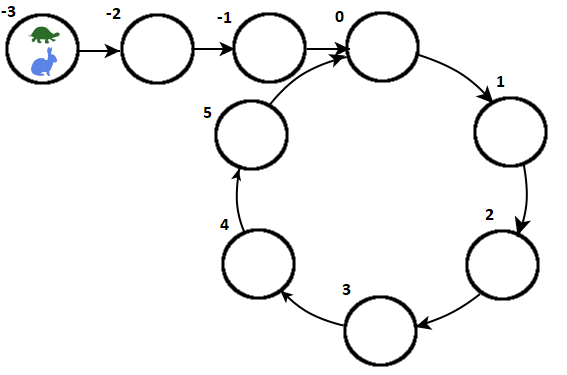
\includegraphics[scale=0.5]{Floyd.png}
          \caption{Algorithme de Floyd avec $T=3$ et $C=6$}
        \end{figure}

        La tortue commence en position $-T$, il lui faut précisément $T$ étapes pour qu'elle se trouve au début du cycle, soit en position $0$. A ce moment, le lièvre a avancé de $2 \cdot T$ pas, et il a déjà parcouru $T$ nœuds dans le cycle. Sa position dans celui-ci est donc donnée par le reste de la division euclidienne de $T$ par $C$.

        \begin{align*}
          \exists k \in \mathbb{N} \text{\ tel que } T = C \cdot k + r \text{\, avec } 0 \leq r < C, \text{d'où } T &\equiv r \text{\ mod } C
        \end{align*}

        Lorsque la tortue atteint pour la première fois le nœud $0$, le lièvre est alors en position $r$ dans le cycle. Si $r=0$, c'est terminé, car alors le lièvre et la tortue sont au même endroit. Supposons $r$ différent de $0$. On peut terminer en $C-r$ étapes supplémentaires.

        À l'issue de ces $C-r$ étapes, la tortue est en position $C-r$ dans le cycle. La position du lièvre est donnée par~:

        \begin{align*}
          r + 2 \cdot (C - r) &\equiv 2 \cdot C -r \text{\ mod } C \\
                              &\equiv C - r \text{\ mod } C
        \end{align*}

        Le lièvre et la tortue sont donc au même endroit et il y a collision, on peut trouver un indice $i$ tel que $x_i = x_{2i}$. De plus, on a pu terminer en $T + C - r$ étapes.

        \begin{align*}
          \text{Or } T + C - r &= C \cdot k + r + C - r \\
                               &=(k + 1) \cdot C
        \end{align*}

        \begin{alignat*}{2}
          \text{D'autre part } C \cdot k &< C \cdot k + r &&< C \cdot (k + 1) \\
                         \iff  C \cdot k &< \ \ \ \ \ T   &&< C \cdot (k + 1) \\
        \end{alignat*}

        Donc la première collision a lieu à l'étape $n$, où $n$ est le plus petit entier multiple de $C$ avec $T < n$.
 % Algorithme p de Pollard "classique"
\chapter{Implémentation «\texorpdfstring{\,}{\ }classique\texorpdfstring{\,}{\ }»}
    Dans la partie précédente, nous avons discuté de la méthode de Pollard (telle que présentée dans le \textit{Handbook of Applied Cryptography}~\autocite[106]{handbook}) pour résoudre le problème du logarithme discret.

    Un des objectifs de ce projet est de produire un programme capable de résoudre le problème, que l'on peut formaliser de la façon suivante.

    En appelant le programme sur des entiers $p, q, g, h$ respectant~:
    \begin{equation} \label{eq:2}
      \begin{split}
        p \text{\ et } q \text{\ deux nombres premiers} \\
        \text{tels qu'il existe un unique sous-groupe de } {(\mathbb{Z}/p\mathbb{Z})}^* \text{\ d'ordre } q \\
        g \text{\ un générateur de ce groupe multiplicatif, \textit{i.e} } {(\mathbb{Z}/p\mathbb{Z})}^* =\ < g > \\
        h \in {(\mathbb{Z}/p\mathbb{Z})}^*
      \end{split}
    \end{equation}

    Cette dernière condition assure qu'il existe $x \in \mathbb{Z}$ tel que $h = g^x$; ce $x$ correspond à $\log_g(h)$, et c'est ce que l'algorithme retourne.

    Pour des raisons de performances, ce programme est écrit en C.
    Cependant, afin de se familiariser avec la méthode, et nous assister dans la génération de grands nombres $p$, $q$ et d'un générateur $g$ leur correspondant, nous avons commencé par utiliser le logiciel SageMath\footnote{\url{https://www.sagemath.org/}}. De plus, nous avons aussi pu automatiser la génération de données de tests (des entiers $h$ et $x$ respectant $g^x = h$) pour valider le bon fonctionnement du programme, mais aussi mesurer les performances des algorithmes utilisés, afin de pouvoir mettre en perspective d'éventuelles optimisations dont il sera question plus tard.

    Dans ce chapitre, nous allons donc présenter brièvement le premier prototype que nous avons obtenu à l'aide de Sage.
    Bien que non optimisé, cela nous a permis de découvrir quelques questions et contraintes auxquelles nous avons aussi dû répondre lors de l'implémentation en C.
    Nous parlerons de ces problématiques, en particulier de la génération de grands entiers définissant les groupes dans lesquels nous avons travaillé (pour tester et mesurer l'efficacité de notre programme).
    Enfin, nous présenterons le code C ayant permis de générer notre programme de résolution du problème, ainsi que les différents tests et mesures mis en place pour en valider le bon fonctionnement et l'efficacité.


    \section{SageMath}
        \subsection{Prototype de la méthode \texorpdfstring{$\rho$}{Rho}}
        Pour nous aider à prendre en main la méthode, il nous a été proposé de l'implémenter dans un premier temps à l'aide de Sage.

        Nous nous sommes donc appuyés sur les valeurs données dans le Handbook pour tester notre solution.
        Dans les exemples qui vont suivre, nous nous placerons donc dans le sous-groupe de ${(\mathbb{Z}/383\mathbb{Z})}^*$ d'ordre $191$ et dont $2$ est un générateur.

        Dans les grandes lignes, notre programme Sage s'articule autour de trois fonctions~:
        \begin{itemize}
            \item La fonction \lstinline{f} d'itération.
            \item La fonction \lstinline{rho_table}~: appelle la fonction d'itération jusqu'à détecter une collision (en suivant l'algorithme de Floyd\footnote{Présenté en section~\ref{chapter1:Floyd}.}). Notons que cette fonction stocke l'ensemble des valeurs intermédiaires calculées dans un tableau, pour valider visuellement la correspondance entre la table donnée dans le \textit{Handbook}~\autocite[107]{handbook} et les valeurs que l'on obtient.
            \item La fonction de calcul du logarithme discret recherché (sobrement nommée \lstinline{solve}) en fonction des exposants obtenus lors de la collision.
        \end{itemize}

        Notons que ce code est critiquable sur plusieurs points.

        Premièrement, nous n'avons pas cherché à optimiser notre programme, avons mal architecturé les différentes briques logiques, et n'avons porté aucune attention à la gestion mémoire.
        On note donc, parmi les points problématiques de cette implémentation~: mélange des fonctions de calcul et d'affichage et stockage non nécessaire des valeurs intermédiaires (impliquant probablement, dès lors que l'on utilisera de grands nombres, une consommation mémoire démesurée, et des temps de calculs interminables).

        C'est pour contrôler aux mieux ces aspects que nous nous sommes tournés vers le langage C pour implémenter une version efficiente de l'algorithme de Pollard.

        Finalement, obtenir rapidement un prototype de notre solution à l'aide de SageMath nous a permis de soulever ces questions d'organisation du code et d'esquisser l'architecture dont nous aurons besoin lors de l'implémentation en C.
        Mais avant d'entrer dans ces subtils détails, présentons maintenant un autre sujet pour lequel SageMath a été pertinent~: la génération des nombres $p, q, g, h$ respectant les relations définies en \eqref{eq:2}.

        \subsection{Génération de données}
        \label{chapter2:sagemath:data}
        Pour pouvoir tester et comparer nos futures implémentations en C, nous devons générer un ensemble de données.

        Dans un premier temps, nous allons générer des entiers $p, q, g$ représentant le sous-groupe de $\mathbb{Z}/p\mathbb{Z}$ d'ordre $q$ et engendré par $g$, où $p$ et $q$ sont premiers.

        Nous avons choisi de créer un tel groupe grâce à une fonction prenant en paramètres la longueur binaire de $p$ et de $q$.

        Pour ce faire, on choisit tout d'abord $q$ aléatoirement de $k_q$ bits jusqu'à obtenir un entier $q$ qui soit premier (fonction gen\_order).

        Ensuite, on construit $p$ tel que $q$ divise $p - 1$, ce qui assurera le fait qu'il existe un unique sous-groupe de $\mathbb{Z}/p\mathbb{Z}$ d'ordre $q$. Or on a cela si et seulement s'il existe $u \in\mathbb{Z}$ tel que $p = uq + 1$. Si on veut $p$ de $k_p$ bits, on tire $u$ (toujours aléatoirement) de $k_p - k_q$ bits jusqu'à trouver $p = uq + 1$ premier (fonction gen\_modulus).

        On obtient ainsi un sous-groupe $\mathbb{Z}/p\mathbb{Z}$ d'ordre $q$.

        Pour finir, il nous reste à trouver un générateur de ce groupe ainsi formé. On sélectionne un élément $v \in \mathbb{Z}/p\mathbb{Z}$ (concrètement on commence à $v = 2$). On pose alors $g = v^u \text{ mod } p$. Si $g = 1$, on prend un autre élément $v$ (ou on incrémente $v$), sinon $g$ est un générateur du groupe (fonction gen\_group).\\
        En effet, dans ce dernier cas on aura~:
        \begin{align*}
        g^q & = v^{uq} \\
            & = v^{p-1} & \text{ puisque } p = uq + 1 \\
            & = 1 \text{ mod } p & \text{ d'après le petit théorème de Fermat}
        \end{align*}
        Et cela garantit que $g$ est un générateur du sous-groupe de $\mathbb{Z}/p\mathbb{Z}$ d'ordre $q$.\\

        Maintenant que nous avons créé un groupe comme nous le souhaitions, nous allons construire, pour un groupe donné, plusieurs entiers (100 dans notre cas) $h$ et $x$ tels que $g^x = h$ mod $p$. Dans la mesure où nous aurons ce $x$, nous pourrons alors vérifier que nos algorithmes de résolution du problème du logarithme discret rendent bien le résultat attendu.

        Pour cela nous choisissons simplement $x$ aléatoirement, pour ensuite poser $h = g^x$ mod $p$. Notre fonction gen\_data répète ce procédé 100 fois pour ensuite nous retourner ces données.\\

        À présent, grâce à cette dernière fonction, nous pouvons générer un fichier contenant un ensemble de $p, q, g, h, x$ (un par ligne). C'est ce pour quoi nous avons créé la fonction gen\_test\_inputs. Cette fonction construit des groupes d'ordres $q$ de 5 à 55 bits. Pour un $q$ donné de $k_q$ bits, nous prenons un $p$ de $k_q + 10$ bits et avons donc pour chaque couple $(p,q)$ 100 valeurs de $h$ en appliquant la fonction gen\_data.

        Avec ceci, nous pourrons mesurer les performances moyennes de notre programme sur en fonction de la taille de $q$. Dans la prochaine section de ce chapitre, nous parlerons finalement de notre implémentation en C de la résolution du Logarithme Discret, et en présenterons les performances sur le jeu de données que nous venons de générer.

        \section{Implémentation en C}
          Pour l'implémentation de l'algorithme $\rho$ de Pollard en C, nous avons utilisé la bibliothèque GMP\footnote{\url{https://gmplib.org/}}. Cette bibliothèque introduit un nouveau type~: mpz\_t, qui permet de manipuler de grands entiers. Ce type est un peu contraignant à utiliser~: en effet, chaque utilisation d'un mpz\_t doit s'accompagner d'une initialisation (fonction mpz\_init) et d'un "nettoyage" (fonction mpz\_clear). En outre, chaque opération sur des mpz\_t se fait grâce à une fonction prédéfinie~: par exemple, une addition de deux mpz\_t ne se fait pas avec un simple "+", il faut utiliser la fonction mpz\_add. Aussi, nous devons à chaque fois faire une opération après l'autre~: chaque fonction fait une opération entre deux mpz\_t (ou un mpz\_t et un int), mais pas plus.\\

          Par ailleurs, lorsque nous utilisons les mpz\_t, nous avons choisi de passer par des pointeurs afin d'éviter des copies en mémoire inutiles lors de différentes opérations, et cela permet évidemment un gain de temps.\\

          Dans le but de résoudre le problème du logarithme discret, nous avons implémenté plusieurs fonctions, en nous appuyant sur ce que nous avons écrit dans le premier chapitre~:

          \begin{itemize}
            \item La fonction d'itération $f$ (module iteration\_basic.c~\footnote{Disponible \href{https://github.com/Pamplemousse/pollard_rho_algorithm/blob/master/c/iteration_basic.c}{ici}.}) décrite en~\ref{chapter1:iteration_basique}, avec $S_1 = \{ x_i \equiv 1 \text{ mod } 3 \}$, $S_2 = \{ x_i \equiv 0 \text{ mod } 3 \}$ et $S_3 = \{ x_i \equiv 2 \text{ mod } 3 \}$. Étant donnés $x_i$, $a_i$ et $b_i$, elle calcule les termes suivants.
            \item La fonction de détection de cycle de Floyd $collision$ (module collision\_floyd.c~\footnote{Disponible \href{https://github.com/Pamplemousse/pollard_rho_algorithm/blob/master/c/collision_floyd.c}{ici}.}) comme vue en~\ref{chapter1:Floyd}~: à partir d'un couple $(x_i, x_{2i})$, elle calcule grâce à la fonction d'itération $f$, $x_{i+1} = f(x_i)$ et $x_{2(i+1)} = x_{2i+2} = f(f(x_{2i})$, et on s'arrête lorsque l'on trouve $j \in \mathbb{N}$ tel que $x_j = x_{2j} \text{ mod } p$ et $b_j \neq b_{2j} \text{ mod } q$.
            \item La fonction de résolution du problème $discrete\_log\_from\_exponents$ (module equation\_solver.c~\footnote{Disponible \href{https://github.com/Pamplemousse/pollard_rho_algorithm/blob/master/c/equation_solver.c}{ici}.}) utilisant~\eqref{eq:résolution}~: en partant d'un couple obtenu avec la fonction précédente, elle nous rend $\log_g(h)$.
      \end{itemize}


    \section{Tests et mesures}
      Une bonne pratique de développement logiciel consiste à écrire des tests automatisés visant à valider le bon comportement de tout ou partie d'un programme sous certaines conditions et entrées.

      Afin de valider le bon fonctionnement de ce que nous avons produit, nous avons donc mis en place une suite de tests
      \begin{enumerate*}
        \item unitaires \footnote{Visant à valider le fonctionnement des différents modules du logiciel, en vérifiant par exemple le résultat de fonctions sur des entrées spécifiques.}
        \item d'intégration\footnote{Validant le fonctionnement de l'ensemble du programme ; en vérifiant en particulier des résolutions de logarithme discret sur des entiers produits par exponentiation (dont nous connaissons donc le résultat).}
      \end{enumerate*}
      que nous avons écrits.

      Lorsque l'on écrit des tests, il est intéressant d'avoir à l'esprit qu'ils devraient respecter certaines propriétés, connues sous l'acronyme FIRST :
      \begin{itemize}
        \item Fast : les tests s'exécutent rapidement (et il est donc agréable de les lancer régulièrement).
        \item Isolated ou Independent : les tests ne sont pas reliés entre eux, ne contiennent pas d'effets de bords affectant les autres. Nécessaire pour tester de petite unités de notre programme de façon isolée.
        \item Repeatable : les tests produisent toujours le même résultat étant donnée une même entrée. Cela permet de favoriser l'automatisation des tests et d'avoir confiance en ce qui a été testé auparavant.
        \item Self-validating : les tests détectent quand ils passent ou ratent ; il n'est pas nécessaire de forcer un pauvre programmeur à lire des tonnes de logs pour en connaître le résultat.
        \item Timely : les tests sont écrits au même moment que le code qu'ils valident.
      \end{itemize}

      Nous avons donc, au cours du projet, écrit nos propres tests en C (se compilant et s'exécutant comme des programmes à part entière), intégré les tests qui ont jalonné nos avancées, et finalement automatisé des tests plus exotiques \footnote{Écrits en Bash, nous permettant de manipuler facilement les entrées et sorties standard lors de l'appel à l'exécutable produit.}, que nous placerons sous le label "Tests d'intégration" faute de mieux.

      Ces "Tests d'intégration" nous permettent d'assurer la non régression de notre logiciel lorsque nous en changeons le code. En effet, si les tests passent, c'est que le logiciel calcule correctement le logarithme discret sur les entrées pré calculées. Si on modifie notre code (pour introduire une optimisation ou utiliser un autre algorithme), il nous suffit de lancer les tests pour garantir que notre nouveau programme fonctionne (au moins) aussi bien que le précédent.

      Enfin, comme nous souhaitions mesurer et comparer l'efficacité des algorithmes que nous avons implémenté, nous discuterons du "protocole" que nous avons mis en place pour recueillir et traiter les données relatives aux performances de notre programme.


      \subsection{Tests unitaires}
      Comme nous venons brièvement de le présenter, une grande partie de nos tests a consisté en l'écriture de tests "unitaires", validant le fonctionnement de fonctions uniques, sous certaines conditions et paramètres d'entrée spécifiques.
      Sous forme de programme C, chaque jeu de test est contenu dans un fichier et charge le module qu'il est sensé valider. Ensuite, grâce à quelques macros, nous validons le comportement des fonctions dudit module sous différents paramètres.
      Ainsi, et grâce au découpage modulaire de notre programme, nous pouvons attester du bon fonctionnement individuel des différentes fonctions nécessaires à la résolution du logarithme discret.

      Par exemple, ce test permet de valider que la fonction \lstinline{f} retourne un code d'erreur (-1) si le premier paramètre est un pointeur nul~:

      \lstinputlisting[language=C,firstline=32,lastline=36]{code/test_iteration_basic.c}


      \subsection{Tests d'intégration}
      Malheureusement, valider individuellement le comportement de nos fonctions sur certaines entrées ne garantit pas que lorsqu'elles seront utilisées ensemble, le programme se comportera comme nous le souhaiterions.
      Pour se protéger des bugs qui peuvent alors subvenir, nous avons choisi d'écrire des tests de plus "haut niveau", qui valident les sorties du programme sur des entrées contrôlées.

      Clairement, l'idée est la même que pour les tests unitaires : il s'agit de vérifier le comportement du logiciel (au lieu d'un module) sur des entrées prédéfinies. Comme nous interagissons avec notre programme à travers l'interface en ligne de commande (comme vu en section \ref{}), nous avons choisi d'utiliser un outil nous permettant d'écrire des tests en Bash : bash\_unit \footnote{\url{https://github.com/pgrange/bash_unit}}.

      \begin{sloppypar}
        Le code de ces tests est disponible à l'adresse : \url{https://github.com/Pamplemousse/pollard_rho_algorithm/blob/master/c/test/test_pollard_program.sh}.
      \end{sloppypar}

      Ce test s'appuie sur les données générées par la fonction \lstinline{gen_data}, présentée dans la section~\ref{chapter2:sagemath:data}. Pour rappel, ces données consistent en un ensemble de lignes, chacune formatée comme suit : "$p$ $q$ $g$ $h$ $x$", et respectant $h = g^x$ mod $p$.

      Pour chacune de ces lignes, on formate une entrée que notre programme peut reconnaître, puis on l'exécute sur cette entrée, et enfin, on vérifie que le résultat rendu est conforme à ce que l'on sait être la solution du problème sur notre entrée.
<<<<<<< 9a3b987e9ef4981e1b5b085d1e04c680693d43f8
      Ayant généré beaucoup (plus de 200) de ces solutions, en se plaçant sur différents groupes (en faisant varier $p$ et $q$), nous sommes confiant de la santé de notre programme lorsque ces tests passent~: il est capable de calculer correctement des logarithmes discrets.
=======
      Ayant généré beaucoup (plus de 200) de ces solutions, en se plaçant sur différents groupes (en faisant varier $p$ et $q$), nous sommes confiant de la santé de notre programme lorsque ces tests passent : il est capable de calculer correctement des logarithmes discrets.
>>>>>>> [Rapport] Chapitre 2 : Implémentation en C


      \subsection{Mesure de l'efficacité des algorithmes}
      L'intérêt d'implémenter différents algorithmes d'itération et de détection de collision est de pouvoir comparer leurs performances lors du calcul de logarithmes discrets. Nous ne parlerons pas ici de performance en terme de temps (rapidité d'exécution), ni en terme d'espace (quantité de mémoire utilisée), mais nous cherchons plutôt à évaluer le nombre d'appels à la fonction d'itération (on parlera de nombre de cycles) nécessaires en moyenne avant d'obtenir une collision nous permettant de résoudre le problème.

      À partir d'un jeu de données généré comme expliqué dans la section~\ref{chapter2:sagemath:data}, nous avons exécuté notre programme sur différentes entrées, tout en mesurant, lors de chaque résolution, le nombre d'appels à la fonction \lstinline{f} (fonction d'itération) qu'il a été nécessaire d'effectuer avant l'obtention d'une collision.

      Pour nous permettre de mesurer le nombre d'appels à une fonction spécifique dans notre programme, nous avons utilisé GPROF\footnote{\url{https://sourceware.org/binutils/docs/gprof/}}, en compilant notre programme avec les options \lstinline{-pg -no-pie}. Ces options rajoutent des instructions dites "d'instrumentation", qui permettent de collecter des données lors de l'exécution du programme.
      Ainsi, lorsque l'on lance le programme sur une entrée spécifique, un fichier \lstinline{gmon.out} est généré contenant les données de profilage relative à l'exécution qui vient de se passer. Alors, il nous suffit d'utiliser l'utilitaire \lstinline{gprof} pour en extraire ce qui nous intéresse : le nombre d'appels à la fonction d'itération \lstinline{f}, avec la commande suivante~:

      \begin{lstlisting}
        gprof ../c/pollard -b --exec-counts=f
      \end{lstlisting}

      La figure~\ref{fig:generate_measurement_data} nous montre comment nous avons utilisé ce procédé pour prendre des mesures de façon automatique sur le jeu de données que nous avons généré dans la section~\ref{chapter2:sagemath:data}\footnote{Pour rappel, nous avons généré 51 valeurs de $q$ (de taille variant de 5 à 55 bits), pour lesquelles nous avons trouvé un générateur, puis calculé 100 entrées pour le problème du logarithme discret (par exponentiation à une puissance aléatoire). Au total, notre fichier de test contient donc 5100 lignes contenant les entrées et la solution d'un problème de logarithme discret.}.

      \begin{figure}
        \center{}
        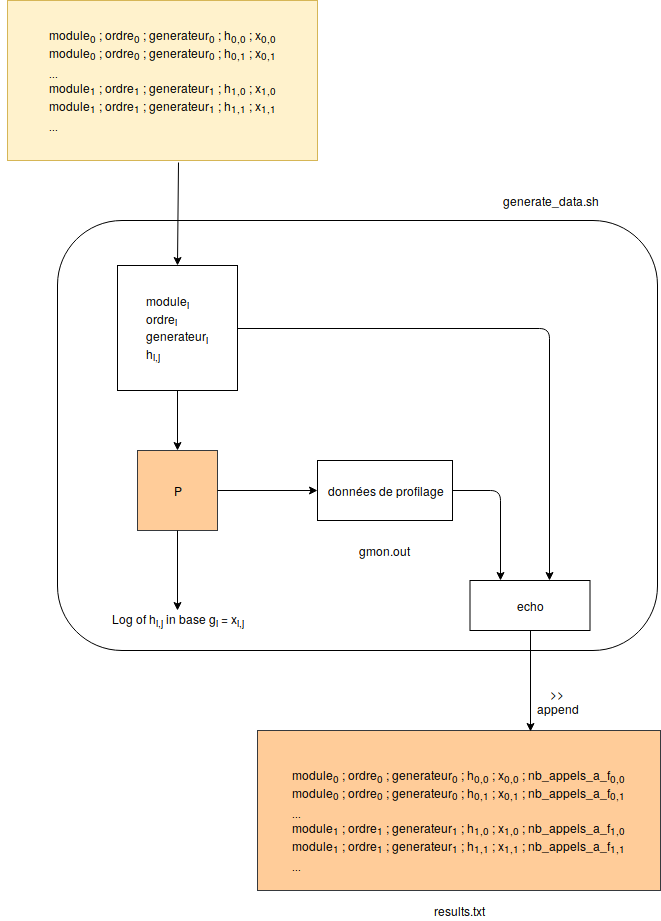
\includegraphics[scale=0.3]{images/generate_measurement_data.png}
        \caption{Agrégation des données générées et des données de profilage}
        \label{fig:generate_measurement_data}
      \end{figure}

      La magie opère à travers le script \lstinline{generate_data.sh}\footnote{Disponible à l'adresse~: \url{https://github.com/Pamplemousse/pollard_rho_algorithm/blob/master/graph/generate_data.sh}}.
      Pour chaque ligne de notre fichier de données, on formate une entrée pour le programme \lstinline{pollard}, dont on profile l'exécution.
      Alors, on récupère le nombre d'appels à la fonction d'itération comme nous venons de le voir, et on ajoute une ligne à notre fichier de sortie suivant le format~: données d'entrées auxquelles on rajoute le nombre que nous venons d'extraire.

      Finalement, nous pouvons traiter les données ainsi recueillies à l'aide de Python et de la librairie Plotly\footnote{\url{https://plot.ly/}} afin d'afficher les résultats obtenus sous forme de graphe.

      Le graphe~\ref{fig:basic_iteration_results} montre les résultats obtenus par notre programme implémentant la méthode de Pollard "originelle", telle que nous l'avons présentée au cours de ce chapitre : utilisant la fonction d'itération présentée dans le \textit{Handbook}~\autocite[107]{handbook} et la méthode du lièvre et de la tortue pour la détection de collisions.

      On peut voir sur ce graphe que la complexité calculatoire de l'algorithme est en $\mathcal{O}(\sqrt{q})$, ce qui confirme les résultats présentés dans le papier originel : \textit{Monte Carlo Methods for Index Computation}\autocite{pollard0}.

      \begin{figure}
        \center{}
        \includegraphics[scale=0.5]{images/iteration_de_base.png}
        \caption{Nombre d'appels à la fonction d'itération avant la détection d'une collision en fonction de la taille de $q$ (l'ordre du groupe)}
        \label{fig:basic_iteration_results}
      \end{figure}


    \paragraph{}
    A présent que nous avons présenté le travail effectué relatif à la méthode de Pollard telle que présentée dans le \textit{Handbook}~\autocite[106]{handbook}, ainsi que les tests et mesures mis en place pour assurer sinon la qualité, au moins le bon fonctionnement de notre implémentation, nous allons dans le prochain chapitre discuter des améliorations possibles à travers de nouveaux algorithmes pour la fonction d'itération, la détection de collision ou la combinaison des deux.
 % Implémentation "classique"
\chapter{Optimisations}
	Cette partie est consacrée à l'étude et à l'implémentation de quelques améliorations possibles pour l'algorithme $\rho$ de Pollard.

		\section{r-adding walks}
    À titre de rappel, l'algorithme $\rho$ de Pollard utilise une fonction d'itération $f$ afin de définir une séquence $(x_i)_{i \ge 0}$ par $x_{i+1} = f(x_i)$. Or, pour obtenir un résultat optimal, il faut que cette séquence ressemble le plus possible à une marche aléatoire. Cela signifie essentiellement deux choses~: la première, c'est que la valeur initiale de la séquence devrait idéalement être un élément choisi aléatoirement dans le groupe $G$ ; la deuxième, c'est que la fonction $f$ devrait être (ou tout du moins se comporter comme) une fonction aléatoire - c'est-à-dire qu'elle devrait résulter d'un choix équiprobable entre toutes les fonctions de $G$ dans $G$. Dans ces circonstances, la méthode $\rho$ de Pollard utilise approximativement $O(\sqrt{n})$ opérations de groupe pour trouver $\log_g(h)$, avec $n$ l'ordre de $G$.

		Un problème majeur est donc la simulation d'une marche aléatoire. L'algorithme $\rho$ de Pollard original ne permet pas d'atteindre les performances d'une telle marche. D'autres méthodes ont donc été développées afin d'obtenir des performances plus proches de celles d'une marche aléatoire. Parmi elles, la variante des r-adding walks, que nous allons étudier à présent.

		Comme pour la méthode originale, il faut commencer par partitionner le groupe $G$ en sous-ensembles d'environ la même taille. On choisit donc un entier naturel $3 \leq r \leq 100$ et on trouve $r$ sous-ensembles $(T_i)_{i \in \{0,\cdots,r-1\}}$ de tailles à peu près équivalentes. On obtient ainsi $G = \bigcup\limits_{i=0}^{r-1} T_i$. On définit la fonction d'indexation $s$ comme suit~:

		\begin{center}

		$\begin{array}{lrcl}
		s : & G & \longrightarrow & \{0,1,\cdots,r-1\} \\
		    & x & \longmapsto & s \text{ si } x \in T_s
		\end{array}$

		\end{center}

		Pour chacun des nombres $s \in \{0,\cdots,r-1\}$, on choisit aléatoirement deux entiers $m_s$ et $n_s$ dans $\mathbb{Z}/q\mathbb{Z}$ et on pose $M_s = g^{m_s} \cdot h^{n_s}$. Enfin, on définit la fonction d'itération $f$ comme $f(x) = x \cdot M_{s(x)}$ et la suite $(x_i)_{i \ge 0}$ par $x_0 = 1$ et $x_{i+1} = f(x_i)$. A présent, montrons que $f$ permet le traçage des exposants par rapport à $g$ et $h$.

		Il faut trouver deux suites $(a_i)_{i \ge 0}$ et $(b_i)_{i \ge 0}$ telles que $x_i = g^{a_i} \cdot h^{b_i}$ pour tout $i$. Posons :

		\begin{align*}
      \begin{cases}
        a_0 = 0 \\
        a_{i+1} = a_i + m_{s(x_i)}
      \end{cases}
    \end{align*}

    \begin{align*}
      \begin{cases}
        b_0 = 0 \\
        b_{i+1} = b_i + n_{s(x_i)}
      \end{cases}
    \end{align*}

		Comme pour la méthode originale de l'algorithme $\rho$ de Pollard, dans quelques rares cas cette fonction d'itération ne permet pas de détecter une collision. Il suffit alors de prendre les entiers $a_0$ et $b_0$ aléatoirement dans l'intervalle $\mathopen{[}1,q-1\mathclose{]}$ et de poser $x_0 = g^{a_0} \cdot h^{b_0}$. On exécute ensuite l'algorithme normalement.

		Montrons par récurrence que ces deux suites conviennent.

		\subsection*{Initialisation}

		Dans le cas général, par définition, $x_0 = 1$, $a_0 = 0$ et $b_0 = 0$. On a donc~:

		\begin{align*}
          g^{a_0} \cdot h^{b_0} &= g^{0} \cdot h^{0} \\
                                &= 1 \cdot 1 \\
                                &= x_0
        \end{align*}

        Dans les quelques rares cas où $a_0$ et $b_0$ sont choisis aléatoirement dans $\mathopen{[}1,q-1\mathclose{]}$, on a $x_0 = g^{a_0} \cdot h^{b_0}$ par définition.

        La relation est donc vraie au rang $0$.

        \subsection*{Hérédité}
        On suppose que la relation est vérifiée pour un $k \in \mathbb{N}$, c'est-à-dire $x_k = g^{a_k} \cdot h^{b_k}$. Montrons que l'on a $x_{k+1} = g^{a_{k+1}} \cdot h^{b_{k+1}}$.

        Par définition $x_{k+1} = f(x_k) = x_k \cdot M_{s(x_k)}$. Par hypothèse de récurrence, on a donc~:

       \begin{align*}
          x_{k+1} &= g^{a_k} \cdot h^{b_k} \cdot g^{m_{s(x_k)}} \cdot h^{n_{s(x_k)}} \\
                  &= g^{a_k + m_{s(x_k)}} \cdot h^{b_k + n_{s(x_k)}} \\
                  &=g^{a_{k+1}} \cdot h^{b_{k+1}}
        \end{align*}

        \subsection*{Conclusion}
        On a montré que la relation est vraie pour $i = 0$, et que si elle est vérifiée au rang $k$, elle l'est aussi au rang $k + 1$. Donc pour tout $i \in \mathbb{N}$, $x_i = g^{a_i} \cdot h^{b_i}$.

        \section{Méthode des points distingués}
        Trouver un moyen de détecter une collision le plus rapidement possible après que celle-ci ait eu lieu est un autre problème important. L'objectif est de limiter au maximum le nombre d'appels à la fonction d'itération avant d'obtenir une collision, tout en utilisant peu de mémoire. Plusieurs méthodes ont été développées ; parmi elles, celle des points distingués de Quisquater et Delescaille est considérée comme la plus efficace.

        On commence par choisir une propriété sur les éléments de $G$ qui soit facilement vérifiable - par exemple, avoir une écriture binaire se terminant par un certain nombre de $0$. Les éléments de $G$ satisfaisant cette propriété sont appelés les points distingués.

        On choisit un élément de $G$ de manière aléatoire et on lance la fonction d'itération dessus. Les appels à cette fonction s'arrêtent lorsqu'on a obtenu un point distingué. Celui-ci est alors stocké dans une table (on stocke également $a_i$ et $b_i$ tels que cet élément de $G$ s'écrit $g^{a_i} \cdot h^{b_i}$), et on choisit un autre élément de $G$ de manière aléatoire avant de réitérer le procédé. L'algorithme s'arrête lorsqu'on a trouvé deux points distingués égaux. Il y a fort à parier qu'on est parti de deux éléments différents de $G$ pour trouver ce point distingué, et que par conséquent on ait trouvé deux écritures différentes du point distingué en fonction de $g$ et $h$. On obtient donc des éléments $a_i$, $b_i$, $a_j$ et $b_j$ tels que $g^{a_i} \cdot h^{b_i} = g^{a_j} \cdot h^{b_j}$ avec $(a_i,b_i) \neq (a_j,b_j)$ et on peut résoudre le problème du logarithme discret.

        Pour que cette méthode fonctionne correctement, il faut choisir la propriété de telle sorte à ce que la table soit de taille manipulable. Cependant, si la propriété fixe quelques bits, alors ces bits n'ont pas besoin d'être stockés dans la table, ce qui permet des économies de mémoire (par exemple, si tous les points distingués se terminent par un même chiffre, inutile de le stocker dans la table). Si on note $\theta$ la fraction des éléments de $G$ satisfaisant la propriété des points distingués, alors l'algorithme doit terminer avec collision après environ $\sqrt{q\pi/2} + 1/\theta$ appels à la fonction d'itération. L'intérêt majeur de la méthode est qu'elle permet le traitement parallèle par plusieurs processeurs, ce qui permet des résultats encore meilleurs.
 % Optimisations

\printbibliography

\end{document}
